\NeedsTeXFormat{LaTeX2e}
\documentclass[11pt,twoside]{book}
\usepackage{parskip}
\usepackage[utf8]{inputenc}
\usepackage[T1]{fontenc}
\usepackage{ae}
\usepackage[intlimits, sumlimits, namelimits]{amsmath}
\usepackage{bbm}
\newcommand{\inp}[1]{\ensuremath{\left(#1\right)}}
\newcommand{\sqr}{\ensuremath{^{2}}}
\newcommand{\cube}{\ensuremath{^{3}}}
\newcommand{\set}[1]{\ensuremath{\mathbbm{#1}}}
\newcommand{\norm}[1]{\ensuremath{\left|#1\right|}}
\newcommand{\vect}[2]{\ensuremath{\inp{\hspace{-.8ex}\begin{array}{c}#1\\#2\end{array}\hspace{-.4ex}}}}
\newcommand{\svec}[3]{\ensuremath{\inp{\hspace{-.8ex}\begin{array}{r}#1\\#2\\#3\end{array}\hspace{-.4ex}}}}
\newcommand{\entspr}{\ensuremath{\,\,\hat{=}\,\,}}%
\newcommand{\dx}[1][x]{\ensuremath{\textnormal d #1}}
\newcommand{\trace}{\textnormal{Tr}}

% For stupid thinkos:
\newcommand{\cross}{\times}
\newcommand{\dell}{\partial}

% make things shorter:
\newcommand{\lso}{\ensuremath{L_{\textnormal{SO}}}}
\newcommand{\tso}{\ensuremath{t_{\textnormal{SO}}}}


\usepackage{array}
\setlength{\extrarowheight}{.2mm}
\usepackage{hyperref}
\usepackage{graphics,graphicx,fancyvrb}

%Raender einstellen
\usepackage[a4paper, inner=35mm, outer=25mm,top=30mm]{geometry}
%\usepackage[a4paper]{geometry}
%\usepackage{lastpage}
\usepackage{fancyhdr}
%	\lhead{Moritz Lenz}
%	\chead{\bfseries{-- \thepage\ --}}
%	\rhead{\thetitle}
%	\lfoot{}
%	\rfoot{}
%	\cfoot{}
%	\pagestyle{fancy}
\pagestyle{plain}

\sffamily

\bibliographystyle{alpha}


\author{Moritz Lenz}
\title{Ballistic Transport of Spin-Polarized Electron Beams in Mesoscopic Systems}
\begin{document}

\begin{titlepage}
% \maketitle 
\begin{center}
    \begin{center}~\\ \vspace{2cm}
    \end{center}
    \begin{huge}
    \textbf{Ballistic Transport of Spin-Polarized\\[0.2em]
        Electron Beams in Mesoscopic Systems}
    \end{huge}
\par
\vspace{3 cm}

\large Diploma thesis by  
\\[1.5em]
{
\LARGE\sc Moritz Andreas Lenz
}
\par
\vspace{1 cm}
\large Supervised by \\[1em]
{
    \sc
Prof. Dr. Ewelina Hankiewicz
}

\vspace{4 cm}

\normalsize A.G. Mesoskopische Physik, Institut f\"ur Theoretische Physik und Astrophysik, \\
Universit\"at W\"urzburg, D-97074 W\"urzburg, Germany

\vspace{2 cm}
~\\ December 18, 2009 % \today
~\\
 
\end{center}
\end{titlepage} 

~\newpage


\tableofcontents
\chapter{Introduction}

Spin manipulation opens up an interesting range of possible applications, from
spin powered nano devices to Quantum Computing and Quantum Cryptography.

A quantum computer works with superposition of quantum mechanical states, and
spin states stay coherent for much longer than change states, so spin states
present a natural alternative to the classical systems which use spatially
separated electron charges to store and manipulate information.

Also in charge based devices -- such as NPN transistors -- charges have to be
moved to change the conduction properties, and moving charge requires energy,
and dissipates heat. Since spin devices are conceivable which do not require
spatial separation to operate, but rather work with flipping spins, they could
be much more energy efficient.

The first measurement of the spin degree of freedom was carried out by O.~Stern
and W.~Gerlach in 1921 \cite{stern-gerlach} and employed a beam of silver atoms,
which were
exposed to a strong, inhomogeneous magnetic field and thus spatially separated
according to their spin orientation.

For building spin based devices, such a setup is hardly feasible. Later
experiments in solids used ferromagnetic materials to generate spin polarized
electron beams. A famous example is the Giant Magneto Resistance, which
enabled much higher storage density in hard disks, and was awarded with the
Nobel Prize in 2007.

Spin manipulation has traditionally been hard to achieve on nanometer
scales. Using ferromagnetic materials, it is possible inject spin polarized
currents into semiconductor structures, and various mechanisms have been
researched to manipulate these spin currents. In 1990 S.~Datta and B.~Das
published their thoughts on how to build a spin-based
transistor \cite{datta-das}.

They proposed two ferromagnetic contacts separated
by a quantum well with tunable spin-orbit coupling. By tuning the spin-orbit
coupling strength, the spin precession length can be controlled, and thus the
spin orientation at the second contact. Since ferromagnetic contacts are
sensitive to spin orientation, the current transmitted through the contacts can be
modulated.

However, building ferromagnetic contacts or devices on
the nano scale is a serious technological challenge, and combining millions of
ferromagnetic structures on a single device seems hardly possible. There is
also a conceptual difficulty: due to the band structure mismatch between
metallic ferromagnetic materials and semiconductors, additional interface
effects (like in Schottky diodes) arise, which can seriously inhibit the
usefulness of such devices.

New hope for non-magnetic spintronic devices came from the experimental
observation of the Spin-Hall Effect in 2004 \cite{SHE}, which was
theoretically predicted in 1971 \cite{dyakonov}. In analogy to the
classical Hall effect, an electrical current causes a spin imbalance in
lateral direction. Unlike the ordinary Hall effect, no magnetic field is
required, but rather the spin assembly is caused by the band
structure of the semiconductor heterostructure, or by impurities.

In this Diploma Thesis, we investigate how a spin polarized electron
beam can be achieved by using only non-magnetic materials. The Rashba 
spin-orbit coupling, which arises from
asymmetric structures in certain semiconductors, can be used as a tunable
means to treat
electrons in a spin-dependent way. In particular, an interface
between regions with different strengths of spin orbit interactions can be
used to split a non-polarized beam into two spatially separated beams of
different spin polarization.

We discuss such interfaces, and also the experimentally more accessible setup
of having two regions with different strengths of spin-orbit coupling.

In particular we look at a nanometer or micrometer sized, two dimensional
electron gas in a semiconductor at zero temperature where electrons and holes
are transported coherently (i.e.~without dephasing) and ballistically
(i.e.~without or with very little scattering). Such electron gases are
experimentally accessible in quantum wells at heterojunctions in GaAs,
HgTe and other semiconductors.

In Chapter \ref{sec:theory} we present the basic theoretical underpinning for
the calculations to come: the Landauer Formula which relates conductance to
the transmission matrix $T$, the Fisher-Lee relation which allows calculation
of $T$ based on the Green's function in sample and lead, the Rashba-Bychkov
spin-orbit coupling which causes all the interesting effects discussed in this
thesis, and finally we present a tight binding model which allows numerical
calculation of the Green's functions and thus $T$.

In Chapter \ref{sec:analytical} we present an analytical model of an electron
wave traveling from a normal region to a region with spin-orbit coupling. The
wave is decomposed into two parts of opposite chirality, and we 
analyze the transmission and reflection coefficients resolved by chirality.
We expand this model to a system where both sides of the interface have
non-zero (but different) spin-orbit interaction.

Chapter \ref{sec:numerics} explains the numerical calculations in depth. We
present the used algorithm and possible alternatives, considerations regarding
the run time performance and numerical errors, and of course results from
these calculations. We find that decent spin polarizations can be achieved
for appropriate interface angles and spin-orbit strengths, even in the new
case where there is non-zero spin-orbit interaction on both sides of
the interface.

We also explain how the results of the analytical calculations can be compared
to the numerical results, and how projection from the chiral bases to the
spin-up/spin-down bases diminishes some of effects of the interfaces.

Chapter \ref{sec:summary} finally summarizes our achievements, and shows up
possible directions in which our models could be expanded.

% vim: spell


\chapter{Theory}
\label{sec:theory}

Consider a two-dimensional conductor of width $W$ and length $L$. If these two
dimensions  are large enough, the conductance is

\begin{align}
    G = \sigma \frac{W}{L}
\end{align}

where $\sigma$ is a material specific parameter and independent of the
geometry of the conductor. \emph{Large enough} means in this context
specifically that both lengths are large compared to all of three
characteristic lengths: the Fermi wavelength, the mean free path and the
phase-relaxation length.

The mean free path is the average distance which a charge carrier can travel
before it is scattered (by an impurity, electrons or phonons) and thus loses
momentum.

If the length of the conductor is smaller than the mean free path, most
electrons travel through it without scattering, and one could naively assume
that this means the resistance is zero.

Still experiments show that a finite resistance can be observed. That is
because the sample cannot be measured in isolation; it is attached to the
macroscopic measuring system through \emph{leads}. Even if the leads are very
good conductors themselves, a contact resistance arises. So the theory has to
take into account both the sample and the leads.

The following explanations are mostly taken from \cite{datta}.

\section{Landauer Formula}

\begin{figure}
    \begin{center}
        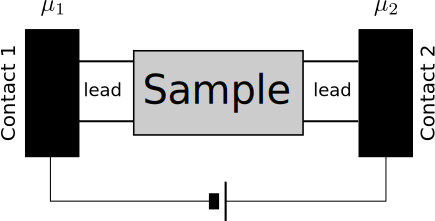
\includegraphics[width=0.5\textwidth]{sample-leads}
    \end{center}
    \caption{Schematic setup to derive the Landauer Formula}
    \label{fig:sample-leads}
\end{figure}

The sample is attached to two leads, which we assume to be perfect, ballistic
conductors with $M$ modes each. We assume that the contacts are
reflectionless, that is electrons can travel from the sample into the contacts
without reflection.

This means that the $k_x$ states in the left lead are occupied by electrons
coming from contact 1 and thus have the same electrochemical potential as
the contact $\mu_1$. Likewise the $-k_x$ states in the right lead have the
potential $\mu_2$.

At zero temperature, only electrons with energies between $\mu_1$ and $\mu_2$
are transported, and the influx from the left lead is
$I_1^+ = (2e/h)M(\mu_1-\mu_2)$. We call the transmission probability through
the sample $T$, so the outflux from lead 2 is $I_2^+ = T I_1^+$, the rest
is reflected back: $I_1^- = (1-T) I_1^+$. The net current $I$ then is

\begin{align}
    I = I_1^+ - I_1^- = \frac{2e}{h} M T (\mu_1 - \mu_2)
\end{align}

The conductance is

\begin{align}
    G = \frac{I |e|}{\mu_1 - \mu_2} = \frac{2 e^2}{h} MT
\end{align}

\section{Transmission and Green's Functions}

To calculate the matrix $T$, one can make use of the so-called \emph{Green's
functions}. A Green's function $G$ is, loosely speaking, an inverse of a
differential operator $D$. More precisely, if the relation between an
excitation $\delta$ and a response $R$ is $D R = \delta$, then every
operator $G$, for
which the equation $R = G \delta$ holds, is called a Green's function.

To calculate the wave function $\psi$ in response to an excitation $\delta$ at a
given energy $E$, we can use the inhomogeneous Schrödinger Equation

\begin{align}
    \label{eq:green-define}
    (E - H) \psi = \delta
\end{align}

where $H$ is the Hamiltonian operator. In a one-dimensional wire oriented
along the $x$ axis with Hamiltonian $H =
-\frac{\hbar^2}{2m}\frac{\partial^2}{\partial x^2}$, we expect an excitation of the form
$\delta = \delta(x - x_0)$ to result in two waves propagating away from $x_0$,
so our ansatz is

\begin{align}
    G(x, x_0) = \begin{cases}
        A^+ e^{i k(x-x_0) } \qquad \textnormal{ for } x > x_0 \\
        A^- e^{-i k(x-x_0) } \qquad \textnormal{ for } x < x_0 \\
    \end{cases}
%    \left\{   \right.
\end{align}

This function satisfies Eqn. \ref{eq:green-define} for every point $x \not=
x_0$  for $ k = \sqrt{\frac{2mE}{\hbar^2}}$.

From the boundary conditions

\begin{align}
    G(x = x_0 + 0, x_0) - G(x = x_0 - 0, x_0) &= 0 \\
    \frac{\partial G(x, x_0)}{\partial x}\left.\right|_{x=x_0 +0}
    -\frac{\partial G(x, x_0)}{\partial x}\left.\right|_{x=x_0 -0}
        &= \frac{2m}{\hbar^2}
\end{align}

(where, by $+0$, we mean \emph{evaluated from the right} and by $-0$ we mean
\emph{evaluated from the left}).

We obtain $A^+ = A^- = -\frac{i}{\hbar v}$ where $v := \frac{\hbar k}{m} $.

We call this particular solution the \emph{retarded Green's function} $G^R$,
to distinguish it from a second solution with opposite sign, both in the $A$s
and in the exponent which we call the \emph{advanced} Green's function $G^A$.

In a wire with finite width multiple modes can propagate, but since we can
separate the $x$ and $y$ components, the Green's functions become only
marginally more complex:

\begin{align}
    G^R(x, x_0) = \sum_m A^\pm_m \chi_m(y) e^{i k_m |x - x_0|}
\end{align}

where the transverse wave functions $\chi_m(y)$ satisfy the Schrödinger
Equation in $y$ direction with eigenvalue $\epsilon_m$.

The orthogonality of the different $\chi_m(y)$ functions and the boundary
conditions give us an expression for the amplitudes:

\begin{align}
    A^\pm = - \frac{i}{\hbar v_m} \chi_m(y_0)
\end{align}

If $E$ is an eigenvalue of $H$, $(E-H)^{-1}$ does not exist. One guards
against such singularities by introducing a small, real number $\eta$ and
defines

\begin{align}
    G^R &= \left( (E + i \eta)\mathbf{1} - H \right)^{-1}\\
    G^A &= \left( (E - i \eta)\mathbf{1} - H \right)^{-1}
\end{align}

where $i$ is the complex unit.

One can (with some approximations) obtain a matrix representation for $H$
(see section \ref{sec:tight-binding}) and thus calculate the inverse, as
long as we only consider closed systems.

\begin{figure}
    \begin{center}
        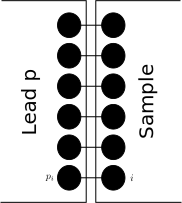
\includegraphics[height=5cm]{coupling-sample-lead}
    \end{center}
    \caption{Coupling between a lead and the sample}
    \label{fig:coupling-sample-lead}
\end{figure}

When we consider a discrete lattice both in the sample and in the leads, we
can couple adjacent lattice points in the sample and a lead as shown in Fig.
\ref{fig:coupling-sample-lead}.

The overall Green's function for both sample and lead can be partitioned into
a Green's function for the sample $G_s$, for the lead $G_p$ and two coupling
Green's functions $G_{sp}$ and  $G_{ps}$

\begin{align}
\left(
    \begin{array}{ll}
        G_p    & G_{ps}\\
        G_{sp} & G_s
    \end{array}
\right)
=
\left(
    \begin{array}{ll}
        (E + i\eta)\mathbf{1} - H_p   & \tau_p\\
        \tau_p^\dagger                & E\mathbf{1} - H_s
    \end{array}
\right)^{-1}
\label{eq:coupling-green}
\end{align}

where $\tau_p$ is the coupling matrix for lead $p$ and contains only non-zero
entries $t$ for matrix elements connecting adjacent sites in lead and sample.

From \ref{eq:coupling-green} we can find an expression for $G_s$:

\begin{align}
    G_s = (E\mathbf1 - H_s - \tau^\dagger g_p^R \tau_p )^{-1}
\end{align}

where $g_p^R$ is the retarded Green's function for the isolated lead $p$,

\begin{align}
    g_p^R = ((E+i\eta)\mathbf1 - H_p)^{-1}
\end{align}

$g_p^R$ can often be calculated analytically. We call the term $\tau^\dagger
g_p^R \tau_p$ \emph{self-energy} $\Sigma^R_p$. Its real part describes the
energy shift of an electron entering the sample, and the imaginary part
determines the life time of a state in the sample.

When multiple independent leads are attached
to the same sample, the effects of the self-energies for each lead simply add
up, and we get

\begin{align}
    G_s^R &= \left(E\mathbf1 - H_s - \sum_p \Sigma^R_p\right)^{-1} \\
    \textnormal{with } \Sigma^R_p &= \tau^\dagger g_p^R \tau_p
\end{align}

It can be shown \cite{fischer-lee,baranger} that the transmission $T_{pq}$ from lead
$q$ through the sample into lead $p$ is

\begin{align}
    T_{pq} = \trace(\Sigma_p G_s^R \Sigma_q G_s^A)
\end{align}

This is called the Fischer-Lee-Relation.

It allows numeric calculation of transmission coefficients for
arbitrary Hamiltonian operators, and is thus independent of the individual
phenomena which we are looking at.

\section{Rashba Spin-Orbit Coupling}

The Dirac equation from relativistic quantum theory describes an electron
coupled to a positron. Since the gap $\Delta = 2 m_e c^2$ is quite large, the
effect of the positron on the electron is very small (at low energies at
least) and can be
taken into account by folding the $4\times4$ Hamiltonian (two dimension to
take spin into account, two for electron and positron) to an effective
$2\times 2$ Hamiltonian.

One of the terms in the Pauli equation resulting from this folding is the
\emph{Pauli Spin-Orbit coupling} term \cite{winkler2003}

\begin{align}
    \left( \frac{\vec p^2}{2m}- \frac{e\hbar \ \vec\sigma \cdot (\vec p \times \vec E)}
                    {2\Delta} +\ldots\right)\Psi = E \Psi
\end{align}

where $\vec E$ is the electric field and $\vec \sigma$ is the vector
which contains the Pauli matrices.

In solids, the coupling takes place between holes and electrons. Since the
energy difference between the bands $G$ can be in the order of meV or eV
(as opposed to $\Delta \approx 1GeV$ for electrons in vacuum), the spin orbit
coupling strength can be as much as one million times higher
than in vacuum.

In a solid in equilibrium, any electric field is either part of the band
structure (and thus taken care of by folding down to a reduced Hamiltonian)
or is induced by a structural asymmetry.

In solid state physics, the spin-orbit coupling term due to structural
inversion asymmetry is called \emph{Bychkov-Rashba} term or simply
\emph{Rashba} term (after \cite{rashba}) and is usually written as

\begin{align}
    H = \frac{\vec p ^2}{2m^*} + \alpha \inp{\vec I \times  \vec \sigma} \cdot \vec p
\end{align}

where $\vec I$ is a unit vector pointing into the direction of the asymmetry,
$m^*$ is the effective mass
and $\alpha$ denotes the strength of the spin-orbit coupling.

\begin{figure}[tb]
    \begin{center}
        \includegraphics[height=0.5\textwidth]{rashba-dispersion.jpg}
    \end{center}
    \caption{The Rashba spin-orbit coupling lifts the spin degeneracy of the
        dispersion relation $E(k)$for $k != 0$. 
        Image courtesy by M. Mühlbauer \cite{mathias}.
    }
    \label{fig:rashba-dispersion}
\end{figure}

This effect lifts the degeneracy of spin-up and spin-down electrons for
$k \not= 0$:

\begin{align}
    E(k) = \frac{\hbar^2}{2 m^*} k^2 \pm \alpha k
\end{align}

So the Rashba spin-orbit coupling splits the spin bands similarly as the Zeeman
effect of a
magnetic field, but it depends on the wave vector and does not come with the
something that is equivalent to the Lorentz force of the magnetic field (see
figure \ref{fig:rashba-dispersion}) .

Since in equilibrium the same number of charge carries have the wave vectors
$k$ and $-k$, the Rashba spin-orbit coupling does not introduce a spin
imbalance, and therefor also no magnetization.


\section{Tight Binding Hamiltonian}
\label{sec:tight-binding}

In order to numerically evaluate the Green's function, we
discretize the sample into sites, and assume that electrons only travel from
one site to an immediate neighbor. This allows us to represent the
Hamiltonian and other differential operators by a finite matrix.


%% TODO: remove bullshit
%% TODO: references
%The nearest neighbor approximation is quite common in transport calculations,
%and comes from the linear combination of atomic orbits (LCAO) ansatz, where
%one assumes that the overlap between localized electron orbitals decreases
%exponentially with distance.
%
%In a two-dimensional square lattice the distance to the next nearest
%neighbors is $\sqrt{2} a$ (where $a$ is the lattice constant), so one can
%approximate that the overlap is $e^{-\sqrt{2}} \approx 0.24$. For a simulation
%that tries to reproduce exact physical behavior of a sample one would have to
%include the next-nearest neighbor hopping, and maybe even one further step
%($e^{-2} \approx 0.14$).
%
%But since our model is an effective one, we have to give up that claim
%anyway, and instead ask ourselves if next-nearest neighbor hopping or higher
%orders contribute any new physics, in terms of symmetries. To the best of our
%knowledge that is not the case, so we keep the nearest neighbor approximation.

For a two-dimensional electron gas with Rashba spin-orbit coupling (of
strength $\alpha$), the Hamiltonian is

\begin{equation}
    H = \frac{1}{2 m^*} (p_x^2 + p_y^2) +
    \frac{\alpha}{\hbar} \inp{p_y\sigma_x - p_x\sigma_y}
\end{equation}

To map this to a discrete lattice, we substitute the derivative by a discrete
difference, so $\dell_x f(x)|_{x_0}$ becomes $(f(x_0+a) - f(x_0))/a$. $a$ is
the lattice constant. For the
second derivative, we chose the symmetric difference $\dell_x^2 f(x)_{x_0} =
(f(x_0+a) - f(x_0-a))/2a$. In the continuum limit $a \mapsto 0$, both reproduce
the derivative exactly.

Written in terms of creation and destruction operators, we obtain

\begin{align}
    H   &= H_0 + H_r\\
    H_0 &= \sum_{n,\sigma} \epsilon_0 c^{\dagger}_{n\sigma} c_{n\sigma}
           - \sum_{n,\delta,\sigma} t c^\dagger_{n\sigma} c_{n,\sigma} +
           \textnormal{H.c.}\\
    H_r &= \frac{-\alpha}{2 a_0} \sum_m
        -i( c^\dagger_{m,\uparrow} c_{m+a_y,\downarrow}
            + c^\dagger_{m,\downarrow} c_{m+a_y,\uparrow})
         + c^\dagger_{m,\uparrow} c_{m+a_x,\downarrow}
            + c^\dagger_{m,\downarrow} c_{m+a_x,\uparrow}
\end{align}

where $n$ runs over all lattice sites, $\delta$ over $\uparrow$ and
$\downarrow$, and $a_x$ and $a_y$ denote the shift to the nearest neighbor in
$x$ and $y$ direction, respectively. (Note that we assume that the lattice is
equally spaced in $x$ and $y$ direction, $+a_x$ just means "go to the next
neighbor in $x$ direction"). $t = \frac{\hbar^2}{2ma}$ is the so-called hopping term, and denotes the
probability of an electron traveling to its nearest neighbor.
$\tso = \frac{\alpha \hbar}{2a}$ is the
Rashba hopping term, and corresponds to a nearest neighbor hop with spin
flip.

Assume we have a quadratic system of $N \times N$ lattice sites.
For a two-dimensional system, we enumerate all lattice sites row by row and
use the result as the index to the Hamiltonian. To incorporate spin, we
identify the indexes that were assigned so far with spin-up and add $N^2$ to
each index to obtain the matrix index for spin-down.

For example, if our system were of size $3 \times 3$, the left-most site in the
first row has index $i = 1$ and the left-most site in the second row has
index $j = N + 1 = 4$ (both spin down). The interaction term (without spin
flip) between these two sites can thus be found at $H_{i,j} = H_{1,4}$. The
interaction that involves a spin flip from $\uparrow$ to $\downarrow$ is
described by $H_{i, j+N^2} = H_{1, 13}$.

\begin{figure}[tb]
    \begin{align*}
        H &= \inp{
           \begin{array}{cc}
                H_{kin}  & H_{spin} \\
                H_{spin}^\dagger & H_{kin} \\
           \end{array}} \\
           %
        H_{kin} &= \inp{
            \begin{array}{ccccccccc}
                -4t & t &  & t\\
                t & -4t & t &  & t &  &  & 0\\
                & t & -4t & 0 &  & t\\
                t &  & 0 & -4t & t &  & t\\
                & t &  & t & -4t & t &  & t\\
                &  & t &  & t & -4t & 0 &  & t\\
                &  &  & t &  & 0 & -4t & t\\
                & 0 &  &  & t &  & t & -4t & t\\
                &  &  &  &  & t &  & t & -4t\end{array}
        } \\
        %
        H_{spin} &= \inp{
            \begin{array}{ccccccccc}
                0 & -\tso &  & i\tso\\
                \tso & 0 & -\tso &  & i\tso &  &  & 0\\
                & \tso & 0 & 0 &  & i\tso\\
                -i\tso &  & 0 & 0 & -\tso &  & i\tso\\
                & -i\tso &  & \tso & 0 & -\tso &  & i\tso\\
                &  & -i\tso &  & \tso & 0 & 0 &  & i\tso\\
                &  &  & -i\tso &  & 0 & 0 & -\tso\\
                & 0 &  &  & -i\tso &  & \tso & 0 & -\tso\\
                &  &  &  &  & -i\tso &  & \tso & 0
            \end{array}
        }
    \end{align*}
    \caption{Tight binding Hamiltonian for $ 3 \times 3 $ lattice sites}
    \label{fig:hamiltonian}
\end{figure}

Figure \ref{fig:hamiltonian} shows an example Hamiltonian for a system of
$3 \times 3$ lattice sites with Rashba spin-orbit coupling (and no magnetic
field).

Sites at the edge of the sample have no hopping element to a neighboring site
at the outside of the sample, so we have hard wall boundary conditions. All
interaction with the outside world is modeled through the self-energy induced
by the attached leads.

\chapter{Analytical Calculations}
\label{sec:analytical}
\newcommand{\ta}{\ensuremath{\tilde \alpha}}
In ref. \cite{khodas}, Khodas et.~al. write about the effects of an
interface between regions of different strengths of Rashba spin-orbit
coupling. We take up their approach and expand on it.

Note that
we use a coordinate system here which differs from the one used in the
rest of this thesis. In particular, we assume the 2DEG in the $x-z$
plane (instead of $x-y$ plane), both for consistency with
ref. \cite{khodas} and because it makes the spinors real vectors and
thus simpler to handle. The results for the $T$ matrix in the end are
the same in both coordinate systems.

\section{Interface Between Normal and Spin-Orbit Coupling Regions}

\begin{figure}
    \begin{center}
        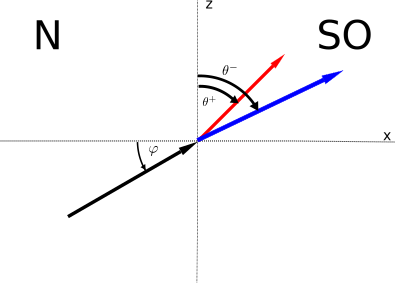
\includegraphics{setup-simple.pdf}
    \end{center}
    \caption{Scheme of the interface between normal (N)
            and spin-orbit (SO) regime}
    \label{fig:setup-zero}
\end{figure}

The setup consists of a 2D electron gas in the $x-z$ plane, where the
strength of the spin orbit interaction is a step function in $x$:
$\alpha(x) = \alpha \Theta(x)$. The region $x < 0$ is called the
"normal region", abbreviated with N, and the region with $x > 0$ is
called the "spin orbit" region, abbreviated as SO (Fig.
\ref{fig:setup-zero}).


The Hamiltonian looks like this:

\begin{align}
    H_r &= \frac{p^2}{2m} + (-\vec y \times \vec \sigma) \cdot
            \alpha(x) \vec p\\ 
    p^2 &= p_x^2 + p_z^2
\end{align}

with the eigenvalues and the velocities

\begin{align}
    E_{\pm} &= \frac{p^2}{2m} \pm \alpha \\
    v_{\pm} &= \frac{\partial E_{\pm}}{\partial p} = \frac{p}{m} \pm \alpha
\end{align}

When a wave travels from the N to the SO region, its energy does not
change. Since its dispersion relation changes, the momentum must also
change. From here on, when we write $p$ we mean the momentum in the N
region. The momentum in the SO region then follows as

\begin{align}
    \label{eq:pso}
    p_{SO}^{\pm} &= m v_F (\sqrt{1 + \ta^2} \mp \tilde \alpha) \\
    \tilde\alpha &= \frac{\alpha}{v_F}
\end{align}

$p_z$ is conserved at the interface.

Since $p_{SO}^+ \not = P_{SO}^-$ for $\ta \not = 0$, we see that
the beam splits up at the interface into two beams of opposite
chiralities and different angles $\theta^+$ and $\theta^-$.

The split up of the beams is approximately proportional to $\ta$:

\begin{align}
    \theta^+ - \theta^- = 2 \ta \tan \phi + O(\ta^3)
\end{align}

Solving the eigenvalue equation leads us to the eigenvectors in the SO
region:

\begin{align}
   \chi_{SO}^{\pm} &= \frac{1}{n_{SO}^{\pm}} 
                      \vect{-p_{x,SO}^{\pm} \pm p_{SO}^\pm}{p_z} \\
    (n_{SO}^{\pm})^2 &= |-p_{x,SO}^{\pm} \pm p_{SO}^\pm|^2 + p_z^2
    \label{eq:chi-so-pm}
\end{align}

where the lower index $x$ means that the value is projected onto the
$x$ axis. The angle between the $x$ axis and the momentum of the
incident wave is called $\phi$, so that $p_x = p \cos \phi$.

Note that, in the N regime, $H$ is a diagonal matrix, and the direction
of the eigenvectors can be chosen with some freedom. We pick
$\chi_N^{\pm} = \lim_{\ta \mapsto 0} \chi_{SO}^{\pm}$ to ensure that
$<\chi_N^+|\chi_{SO}^+> = 1$ holds true at a vanishing interface.



The overall wave function consists of an incident wave, 
reflected and transmitted part. In general, the incident wave can
be decomposed into one with $+$ and one with $-$ chirality, which
propagate and scatter independently. Let us consider the incident $+$
wave:

\begin{align}
    \Psi^+ = e^{i p_z z} * \left\{
        \begin{array}{ll}
            e^{i p_x x} \chi_N^+ + e^{- i p_x x} (\chi_N^+ r_{++} +
                    \chi_N^- r_{-+})    & x < 0\\
            e^{i p_x^+ x} \chi_{SO}^+ t_{++} + e^{i p_x^- x}
            \chi_{SO}^- t_{-+}          & x > 0
        \end{array} \right.
        \label{eq:chiral-wafe-function}
\end{align}

The coefficient $r_{-+}$ is the amplitude with which the incident wave
of $+$ chirality is reflected into $-$ chirality etc., while $t$
coefficients stand for transmission coefficients.

Analog equations can be found for the incident wave with $-$ chirality
by changing all signs that appear either as a subscript or
superscript.

To obtain the values for these coefficients, one has to solve the
boundary conditions at the interface. The wave function is continuous
and the current is conserved, so $\frac{\partial H}{\partial p_x} \Psi$ is also
continuous:

\begin{align}
    \Psi_N|_{x = -0}    &= \Psi_{SO}|_{x = +0} \label{eq:continuous}\\
    \left.\frac{\hat p_x}{m} \Psi_N\right|_{x = -0}
                        &= \left. \left(\frac{\hat p_x}{m} -\alpha \sigma_z\right)
                                \Psi_{SO}\right|_{x = +0}
\end{align}

The second equation can be evaluated with $\hat p_x = -i \partial_x$
(assuming $\hbar = 1$, as done in the rest of the calculation).
Carrying out the derivative (and multiplying by $m$) yields:

\begin{align}
    p_x \chi_N^+ (1 - r_{++}) - p_x \chi_N^- r_{-+}
        =& p_x^+ \chi_{SO}^+ t_{++} + p_x^- \chi_{SO}^- t_{-+} \nonumber\\
         &   - m \alpha \left(  \sigma_z \chi_{SO}^+ t_{++}
                            + \sigma_z \chi_{SO}^- t_{-+} \right)
\end{align}

and dived by  $p_x = p \cos \phi$: 

\begin{align}
    \chi_N^+ (1 - r_{++}) - \chi_N^- r_{-+}
        =& \frac{p_x^+}{p_x} \chi_{SO}^+ t_{++} + \frac{p_x^-}{p_x} \chi_{SO}^- t_{-+} \nonumber\\
         &   - \frac{\ta}{\cos \phi} \left(\sigma_z \chi_{SO}^+
                 t_{++} + \sigma_z \chi_{SO}^- t_{-+} \right)
                                \label{eq:j_continuous}
\end{align}

Equations \ref{eq:continuous} and \ref{eq:j_continuous} have two
components each and can be solved unambiguously. 
The solutions expanded to the first non-zero order in $\ta$ each are

\begin{align}
    t_{++} &= 1 +
            \frac{\ta}{2}\left( \frac{1}{\cos^2\phi} - 1 \right)\\
    t_{-+} &= O(\ta^3)\\
    r_{++} &= \frac{\ta}{2} \tan^2 \phi\\
    r_{-+} &= -\frac{\ta}{2} \tan \phi
\end{align}

and for the incident wave with $-$ chirality

\begin{align}
    t_{--} &= 1 - \frac{\ta}{2} \left( \frac{1}{\cos^2\phi} - 1 \right)\\
    t_{+-} &= O(\ta^3)\\
    r_{--} &= -\frac{\ta}{2} \tan^2 \phi\\
    r_{+-} &= -\frac{\ta}{2} \tan \phi
\end{align}

\begin{figure}[h!tp]
    \includegraphics[width=\textwidth]{zero-plus.pdf}
    \includegraphics[width=\textwidth]{zero-minus.pdf}
    \caption{Transmission and reflection coefficients for the
            incident beam with $+$ (upper) and $-$ (lower) chirality
            and $\ta = 0.1$}
    \label{fig:trans-zero}
\end{figure}

Figure \ref{fig:trans-zero} shows the transmission and reflection
coefficients as a function of the angle $\phi$ of the incident wave.

For increasing $\phi$, the angle of the transmitted beam with $+$
chirality, $\theta^+$, grows even faster. When $\theta^+ >=
\frac{\pi}{2}$, the momentum $p_{x,SO}^+$ is imaginary and no current flows
anymore with $+$ chirality. 

\begin{figure}
    \begin{center}
        \includegraphics[width=0.7\textwidth]{critical-angle.pdf}
    \end{center}
    \caption{Critical angle $\phi_c$ as a function of $\ta$. For $\phi
        > \phi_c$ the wave associated with $t_{++}$ is evanescent.}
    \label{fig:critical-angle}
\end{figure}

The angle $\phi$ for which $\theta^+ =\frac{\pi}{2}$ is called the
critical angle $\phi_c$.

\clearpage
With

\begin{align}
    \cos \phi       &= \frac{p_x}{p}\\
    \cos \theta^+   &= \frac{p_{x,SO}}{p_{SO}}\\
    \theta_c^+      &= \frac{\pi}{2}
\end{align}

it follows that

\begin{align}
    \phi_c          &= -\sin ^{-1}\left(a-\sqrt{a^2+1}\right)
\end{align}

Figure \ref{fig:critical-angle} shows the critical angle as a function
of the spin-orbit coupling strength.

Since the wave with $-$ chirality is transmitted at smaller angles
$\theta^- < \phi$, no critical phenomena arise.

\section{Generalization to two Spin-Orbit Regions}

The system can be generalized to two regions with non-zero spin-orbit
coupling (\emph{SO A} and \emph{SO B}).

\begin{figure}[htb]
    \begin{center}
        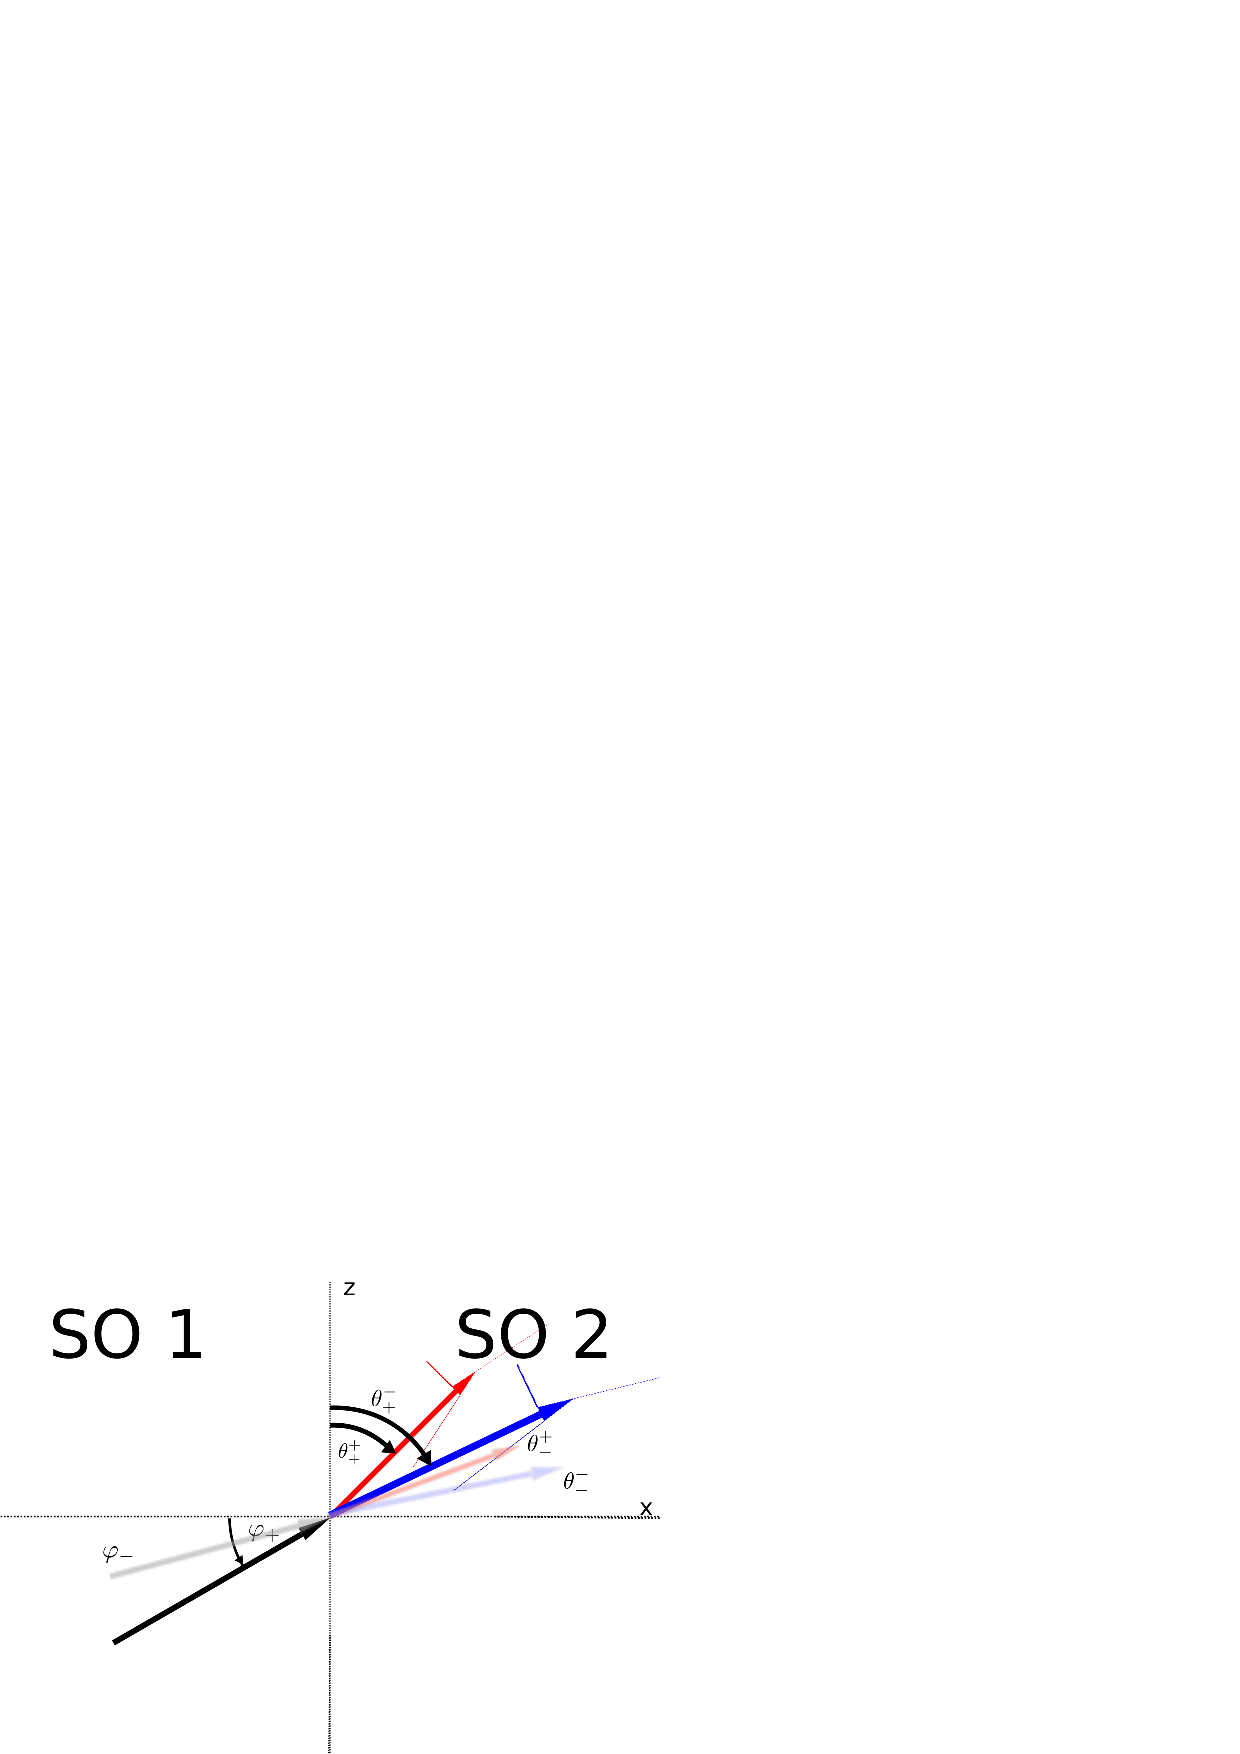
\includegraphics{setup-two-so-regions.pdf}
    \end{center}
    \caption{Scheme of the interface between two regions with
        different, non-zero spin orbit coupling}
    \label{fig:setup-nonzero}
\end{figure}

One just has to remember that the incident beam is split up
into two beams of different chirality, which propagate at different
angles. In general, each beam is split up into two beams at the
interface, so there are up to four beams in \emph{SO B} region,
two of each chirality.

Figure \ref{fig:setup-nonzero} gives an overview of the beams and how
we name them and the associated angles. We will focus our discussion
on the wave with $+$ chirality in the \emph{SO A} region, and the
resulting waves in the \emph{SO B} region.

\begin{figure}
    \begin{center}
        \includegraphics[width=\textwidth]{nonzero-plus.pdf}
        \includegraphics[width=\textwidth]{nonzero-minus.pdf}
    \end{center}
    \caption{Transmission and reflection coefficients for the
        incident $+$ (top) and $-$ (bottom) wave, with
        $\ta_1 = 0.1$ and $\ta_2 = 0.2$.}
    \label{fig:plots-nonzero}
\end{figure}

As before, equations \ref{eq:continuous} and \ref{eq:j_continuous}
apply and can be solved unambiguously. Figure \ref{fig:plots-nonzero}
shows the transmission coefficients as a function of $\phi$ as a
result from these equations.

As before we can identify a critical angle above which the $+$ wave
does not propagate. Instead of using the condition $\theta^+_+ =
\frac{\pi}{2}$ it is easier to look at the momentum directly:

\begin{align}
    p_{x,B}^+ = \sqrt{ p_B^2 - p_z^2} = p \sqrt{(\sqrt{1+\ta_B^2} -
            \ta_B)^2 - \sin^2 \phi^+}
\end{align}

For $p_B^2 < p_z^2$ the mode is evanescent because $p_{x,B}$ is
imaginary. For $p_B^2 = p_z^2$ the angle $\phi^+$ reaches its critical
value, which is only dependent on the strength of the spin-orbit
coupling strength in the right regime:

\begin{align}
    \phi^+_{B,c} = -\sin^{-1}(\ta_B - \sqrt{1+\ta_B^2})
\end{align}

This is the first gray vertical line in figure
\ref{fig:plots-nonzero}, and in the region $\phi < \phi+_{B,c}$ the various transmission and reflection
coefficients look very similar to the case with $\ta_A = 0$.

The second gray line is critical angle associated with $\ta_A$. For
$\phi > \phi^+_{A,c}$ the momentum in $x$ direction $p_{x,A}$ is again
imaginary, just like if we had another interface to a normal region
left of the $A$ region.

%
%\begin{figure}
%    \begin{center}
%        \includegraphics[width=0.8\textwidth]{rpp-zero-point.png}
%    \end{center}
%    \caption{$\phi_0$, the angle for which $r_{++}$ vanishes, as a
%        function of $\ta_1$ and $\ta_2$ (numerically determined)}
%    \label{fig:rpp-zero-point}    
%\end{figure}
%
%For $\ta_2 > \ta_1$ there's a point for which $r_{++}(\phi_0) =
%0$. Figure \ref{fig:rpp-zero-point} shows $\phi_0$ as a function of
%$\ta_1$ and $\ta_2$.

% vim: ts=4 sw=4 expandtab spell spelllang=en_us tw=70



Numerical transport calculations have a huge advantage over the analytical
calculation: once a formalism is implemented, it works for arbitrary
configurations within the limits of the model. However it doesn't generally
supply us with data that enhances physical understanding, so its best use as a
means to expand on analytical calculations which we already understand.

In that spirit we performed numeric calculations, simulating a sample with
Rashba Spin-orbit coupling, and spin-resolved leads attached at the edges.

The calculation follows this rough scheme:

\begin{itemize}
    \item Set up the Hamiltonian $H$
    \item Calculate the self-energy matrices $\Sigma_p$
    \item Calculate the Green's functions $G^A$ and $G^R$ by inverting
          $H + \sum_p \Sigma_p$
    \item Use the Fisher-Lee relation to calculate the transmission matrix $T$
            from $G^R$, $G^A$ and $\Sigma_p$
\end{itemize}

\section*{Performance consideration}

These numeric calculations are computationally expensive. If we simulate a
lattice with a total of $n$ sites, the matrices $H$, $\Sigma_p$, $G^R$ and
$G^A$ are of dimensions $2n^2 \times 2n^2$

\chapter{Summary and Outlook}
\label{sec:summary}

We analyzed the possibilities of achieving spin polarization in a
non-magnetic, microscopic semiconductor. We found that an interface between
normal and Rashba spin-orbit coupling areas splits an electron beam into
components with different chirality, and can be used to manipulate
spin-polarized electron beams similarly to optical light in media with
different optical densities.

           
If the angle between the interface
and the incident beam exceeds a critical angle, the beam with $+$ chirality
ceases to propagate. This effect can be used to obtain a spin imbalance.

We modeled such a system analytically in order to get a good understanding
of the physics, and in an extensible numerical simulation in order to have
maximal flexibility with the choice of parameters and system details.

We developed a method to compare the analytical and numerical results, and in
that course we found that the measurable spin imbalance is partially
damped by fact that the interface separates electron waves by chirality,
not by spin component in $z$-direction.

Still we predict a decent amount of spin-polarization in $z$ direction, which
is directly accessible to experimental verification.

We also discussed the experimental more accessible setup of two regions with
different, non-zero strengths of spin-orbit interaction, and found that such an
interface can also be used to achieve some spin polarization, albeit
of decreasing magnitude when the spin-orbit coupling strengths become similar. 

In both cases a large angle between the incident beam and the interface is
essential for obtaining a decent spin polarization.

We also pointed out that experimental realization is quite possible, and that
similar (but slightly more complex) setups have been grown and etched in HgTe
quantum wells.

Future work in this area could cover the experimental setup of having a strip
of tunable spin-orbit interaction.

There is also another simple extension to our model that would help making
quantitative predictions: when the spin-orbit coupling in an area is tuned by
applying a gate voltage, not only the spin-orbit coupling strength changes,
but also a potential barrier is built up, which scatters electron in a
spin-independent way. Taking these barriers into account will probably not
enhance our understanding of the spin polarization, but is crucial for
obtaining quantitative predictions of the measured signals.

Also in the experiments  magnetic fields are used to focus beams in the
sample, so magnetic field would be a worthwhile addition to our model.

To incorporate more realistic parameters of a particular semiconductor, 
our model could be expanded to use four bands,
the conductance and valance band for each spin direction. This would allow to
make quantitative recommendations on best angle for such an interface.


% vim: ts=4 sw=4 expandtab spell spelllang=en_us tw=78


\chapter*{Acknowledgments}

I'd like to thank Signe for ongoing support and proof reading, my parents for
sustaining, supporting and encouraging me and Ewelina Hankiewicz for
supervision and proof reading.

I'd also like to thank Björn, Dietrich, Jan, Jörg, Rolf, Stefan, Matthias,
Nelly, Mathias and Matthias for interesting and helpful discussion and other
ways of supporting me.

Where would I be without you?

\bibliography{bib}

\end{document}

% vim: ts=4 sw=4 expandtab spell spelllang=en_us tw=78
